\chapter{Reduced precision}
\label{ch:reduced-precision}
Traditionally, computing application are developed to give exact results.
While this is necessary in certains fields (e.g. aerospace), results with a lower
precision is acceptable for multiple types of data.
As~\cite{Cherubin2020-tt} depicts, numerous studies explored the use of lower 
precision data type to perform computation.
It is an interesting strategy as it has the joint potential to reduce hardware 
size, energy cost, and execution time.
In this chapter, we explore (1) the problem definition of \textit{Reduced Precision},
(2) various data formats used to perform reduced precision,
(3) methods to implement reduced precision,
(4) the growth of quantization in Deep Learning,
(5) the current usage of reduced precision within applications,
and (6) tradeoffs from using reduced precision.

\section{Problem definition}
\label{sc:rp-problem-definiton}
The IEEE~754 standard defines two main floating-point formats.
Altough although offering enough precision for most applications, it can also be unecessary precision.
That is, multiple type of application do not benefit from that much precision.
For this reason, a lot of efforts in creating new data formats with lower precision (discussed in~\ref{sc:rp-data-format}).
The idea behind reduced precision is to represent numbers in a data format with 
lower bit witdh; i.e. lower exponent or mantissa.
Similar mixed-precision is a concept that use data formats of different precision within a program allowing better tunning of data format.
The logic complexity of floating points is approximately proportional to the square of the bit width~\cite{Chen2018-an}.
Therefore, lowering the number of bit in a data format also reduce the dye size 
of a chip and, by consequence, the energy cost and computation time for arithmetic operations.

The work done in~\cite{Cherubin2020-tt} surveys a ragne of tools in the fields of reduced precision.
That same study define five challenges that remain to be addressed for reduced precision:
\begin{itemize}
	\item[1.] Identify the code sections where applying reduced precision is beneficial.
	\item[2.] Determine the data type to use base on the application and architecture.
	\item[3.] Estimate, quantify bounds and manage the numerical error introduced by applying reduced precision to an application.
	\item[4.] Measure the overhead from type casting between different data types.
	\item[5.] Develop a tool that benefit a wide range of applications and platforms.
\end{itemize}
The authors of this study claim that without solving those limitations, reduce 
precision will not be sustainable in commercial or open source application and 
will mostly remain an academic subject.
Moreover, the current lack of tools to perform code conversion makes reduced precision
a large development effort.

Overall, the development of a tool that can be applied to multiple use cases and
architectures is an open issue~\cite{Cherubin2020-tt}.

\section{Data formats for reduced precision}
\label{sc:rp-data-format}
Although Chapter~\ref{ch:background} focused primarily on the IEEE~754 Binary data format, many other data format exist.
In this section, we introduce other data types used within reduced precision studies.

Common Deep Learning frameworks such as Tensorflow~\cite{tensorflow2015-whitepaper} and Pytorch~\cite{PyTorch_2019} support mixed-precision through their API.
Both frameworks support the classical IEEE float32 and float16 with the addition to the \textit{bfloat16} introduced by Google Brain~\cite{bfloat16}.
As shown in Figure~\ref{fig:bfloat16}, the bfloat16 is a 16-bit floating point format that use
the same number of bit as the IEEE float32 for its exponent while having shorther bit witdh for its mantissa.
\begin{figure}[b]
	\centering
	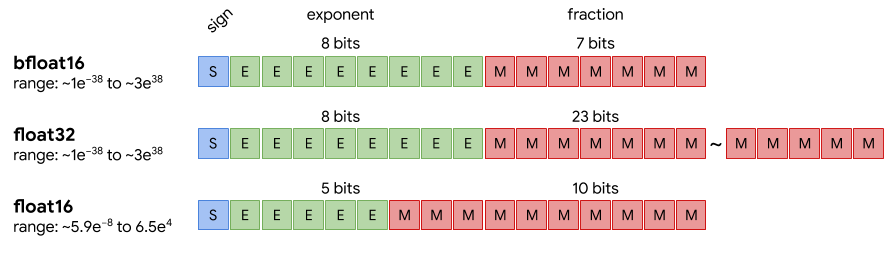
\includegraphics[width=\textwidth]{bfloat16.png}
	\caption{Representation of the bfloat16 floating point format (taken from~\cite{bfloat16}).}
	\label{fig:bfloat16}
\end{figure}
By using the exponent lenght the float32, the blfoat16 allows a quick conversion
data type conversion by dropping, or adding, the extra bits between float32 and bfloat16.
Moreover, with a smaller mantissa size, the hardware chips for the blfoat16 multiplier
is about half the size as the ones for float16 and around 8 times smaller than for float32~\cite{bfloat16}.
Moreover, since Neural Networks (NNs) are far more sensitive to the exponent range than the mantissa,
the blfoat16 performs really as it keeps the exponent range from float32.

Outside of standard Deep Learning frameworks, a variety of different data type were
studied to reduce the precision of machine learning models.
The work from~\cite{Johnson2018-up} evaluates a new \textit{posit tapered} data 
format which combines idea from posit~\cite{Gustafson2017-wo} format and log number system.
Various other studies use different custom floating point formats with reduced 
exponent and mantissa size~\cite{Lesser2011-mn, Chen2018-an, Vicuna2021-mw, Wang2018-oo}.
The authors in~\cite{Carmichael2019-nu} design three FPGAs for low-precision fixed
point, floating point, and posit.

\section{Implementing reduced precision}
% 1 pages
\begin{comment}
- Simulation
- Software and arithmetic implementation
\end{comment}
To remain efficient, consumer hardwares only support a limited set of data formats; for exmaple IEEE~754.
The use of custom data format often requires either: specialized hardware, software implementation, or simulation.

With comodity hardware only supporting the most popular data formats, implementing a new format can be tricky.
A straight forward way to achieve this is to design a custom specialized hardware capable of executing the new format.
The authors in~\cite{Carmichael2019-nu} designed three different FPGAs to support low-precision floats, fixed points, and posits.
Another study~\cite{Johnson2018-up} designed a \SI{28}{\nano\meter} ASIC implement an 8-bit Exact Multiply-Accumulator (EMAC).
On the one hand, the key advantage of designing specilaized hardware is efficiency.
Indeed FPGAs and ASICs, designed for a single tasks can be optimize muc more than a general purpose hardware.
Major hardware manufacturers such as Nvidia and Google design specialized hardware
for frequent Deep Learning tasks (GEMMs), respectively with their recent GPU architectures and TPUs~\cite{tpu}.
On the other hand, creating new hardware is costly both in time and material.
This is especially true when performing study that evaluate a range of different data formats.

% TODO
% Software: Talk about the two papers that use a software implementation.
% Software is not as efficient as hardware; incurs overhead.
% It's also costly to implement and perform code conversion.
% However, it is has the potential to be more portable from one architecture to another.

% TODO
% Simulation: Talk about QPyTorch and the other two papers.
% Simulation is cheap and quick to implement.
% However, it is mostly used to simulation accuracy; performance is hard to simulate.
% Once simulation is done, there needs to be a way to implement it afterwards (either hardware or software).


\section{Growth of quantization in Deep Learning}
% 2 pages
\begin{comment}
- Specify what makes DL a good candidate for RP.
- Describe the different examples in DL. methods, accuracy/performance tradeoff.
- Mention what explain the success of RP in DL and transition to other fields.
- Mention the adoption of RP in other domains.
\end{comment}
In recent years, machine learning, and more specifically Deep Neural Networks (DNNs),
have seen a rise in popularity due to their ability to solve challenging problems.
However, the complexity of DNNs models come with high usage of computing resources.
With the enormous dataset required to train these models, a usual bottleneck is with compute and data communication time.
This motivated multiple studies \cite{Johnson2018-up,Wang2018-oo,Lesser2011-mn,Chen2018-an,Judd2015-kw,Vicuna2021-mw}
to explore the possibility of reducing the precision for the data format used to train those models.
This section explores the quantization methods developed in the Deep Learning 
domain to reduce the compute and data communication of models.

The authors from multiple studies explored the effects of quatization for SVM classification
and found that it is possible to use minimal precision without accuracy loss.
In~\cite{Lesser2011-mn}, the authors investigate the impacts of reducing precision for SVM
classification and estimate the minimal precision required to achieve classification 
without loss of accuracy. Three experiments are performed: 
(1) adding noise to parameters,
(2) using MPFR, simulating reduced mantissa precision from 53 to 4 bits,
and (3) combining the experiment (1) and (2) concurrently.
By comparing the effects of quantization with and without rounding, it is possible To
better isolate the impact of rounding due to reduced precision.
The authors benchmark their experiments on three datasets: SONAR, IRIS, and MUSK.
They use the double precision results as a reference for the classication error.
The results show that lowering the precision up to 15 bits does not affect teh accuracy
for classificatio; this is consistent with the literature.
Further understanding the bounds for reducing the precision would allow to automatically
adjust the precision for classification, which would be an effort towards addressing the third 
challenge from Section~\ref{sc:rp-problem-definiton}.

% \section{Current scope of application}
% % 0.5 page
% \begin{comment}
% - Descirbe how it is currently used and the limitation in term of usability
% - Within framework like PyTorch or Tensorflow, or in academic setting.
% \end{comment}


\section{Tradeoff of using reduced precision}
% 1 pages
\begin{comment}
- Pros
* smaller chip size
* energy saving
* faster computation
* lower storage space
- Cons
* Risk for lower accuracy
* Often requires manual effort to implement/convert
* overhead from casting can be greater than performance benefit
* new data format often require new type of hardware
\end{comment}

